\chapter{}

\begin{figure}
\centering
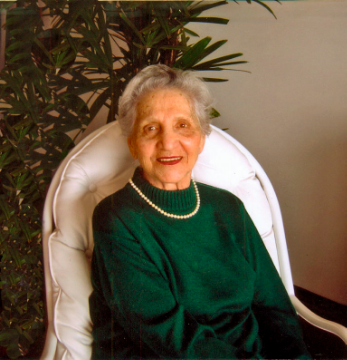
\includegraphics[width=0.6\linewidth]{12/odila.png}
\caption{Tia Odila.}
\end{figure}

Quem conheceu Tia Odila, a irmã mais velha da mamãe, acha que eu me pareço mais com ela do que sua própria filha, Maria Sílvia.
Talvez porque como eu, Tia Odila sempre tenha sido uma mulher grande e forte, obesa até, durante os anos mais difíceis da vida dela.
O corpo generoso, mas bem feito, combinado a uma postura ereta e altaneira comunicava tal impressão de autoridade que ela parecia maior do que de fato era.
Uma gorda elegante.
Mesmo nos seus últimos dias, debilitada pelos sucessivos colapsos do coração, recostada numa poltrona para que o ar não lhe faltasse, esforçou-se por manter a cabeça erguida durante nossa breve conversa e o roupão que envolvia seu corpo definhado ainda era envergado como se fosse arminho.
Ai de mim, essa pose um tanto imperial que a caracterizava, mais de uma vez foi apontada como outro dos traços que nos faziam parecidas.
Mesmo Paulo manifestou muitas vezes o temor de que a semelhança fosse muito além da mera aparência.
Mas, embora admitindo que, como acontecia com ela, muitas vezes minha postura sugeriu às pessoas certo autoritarismo, a identificação nunca existiu além da superfície.
Porque, no meu caso, a atitude servia apenas à causa de vencer a timidez e disfarçar o andar inseguro, mas, no caso dela, havia uma história a justificá-la.

Como Tia Yolanda, Tia Odila foi originalmente educada para voos mais altos do que o árduo e mesquinho caminhar que a vida lhe impôs.
Cedo demonstrou talento para o piano e chegou mesmo a sonhar com uma carreira de concertista, depois que, levada à presença da afamada pianista Antonieta Rudge, ouviu desta os mais calorosos incentivos.
Os estudos lhe custaram sacrifício e paciência porque pianos eram caros e só muito tempo depois de praticar em instrumentos alheios, Tia Odila conquistou o seu.
Já então começara a dar aulas de música para ajudar em casa.
Havia o curso de normalista a pagar no Colégio Mackenzie, pois a Vovó fazia das tripas coração, mas as filhas tinham que estudar em escola particular, na companhia dos rebentos das melhores famílias da cidade.
E havia as duas irmãs menores para vestir e calçar.
Tia Maria Angelina, a caçula, sempre mencionou com gratidão os vestidos e sapatos que a Tia Odila lhe comprava nas melhores casas da cidade, pagando com os magros rendimentos da sua dupla jornada de professora primária e professora de piano.
Já minha mãe não teve essa sorte.
Porque mamãe cresceu em meio à penúria que se seguiu à falência da Mobiliadora que Vovô assumira após a morte do cunhado e, à crise de 1929, que agravou ainda mais a situação da família, jogando o coitado na vala dos desempregados por longos anos.
Durante esse tempo, foi Tia Odila quem assumiu a tarefa de sustentar a casa, secundada pela Vó Didi que dizia rindo, mais tarde, que nesses dias amargos fez de tudo, só não ``fez a vida'', eufemismo que ela usava para designar a atividade do meretrício.
Vovó Didi, todos conhecemos a história, fez sabão, linguiça e pão para vender, deu pensão, costurou para fora, mas nunca sobrava para os vestidos novos com que minha mãe sonhava e muito menos para levar adiante a naufragada carreira de concertista da Tia Odila.
Até o piano teve que ser vendido.

Uma esperança surgiu quando se enrabichou por Odila o belo filho do Coronel Juca Custódio, um dos poderosos da cidade, dono de muitas terras de café.
Cornélio, assim se chamava o jovem herdeiro, era bonito, mulherengo e estroina.
Passava os dias no clube, jogando cartas e as noites nos cabarés da cidade.
Tia Odila tomou a peito, como era bem próprio dela, a tarefa de fazer dele um homem.
Com apoio integral da sogra, Dona Cornélia, lançou-se à missão antes mesmo de subir ao altar.
Mas a empreitada seria muito mais longa e difícil do que supunha.
Sucessivos e variados negócios foram montados antes e depois do casamento na tentativa de conseguir que Tio Cornélio se tornasse um adulto responsável.
Sem sucesso.
Por variadas e sempre muito bem explicadas razões, os empreendimentos não prosperavam.
E tia Odila era quem mais caprichava na defesa do companheiro.
Era mesmo falta de sorte ou conspiração de despeitados.
Nunca alguém ouviu dela, pela vida inteira, qualquer palavra que desabonasse o marido, por mais que os fatos falassem por si.
Tia Odila aprendeu a engolir as decepções e a erguer o queixo voluntarioso na direção inversamente proporcional à frustração que lhe descia goela abaixo.
Dona Cornélia, a sogra, uma aristocrática senhora que eu conheci e que muito me impressionou com seu perfil de camafeu realçado pelo fichú de rendas e coroado por alvos cachos, ensinou-a a cultivar maneiras de uma grande dama.
As bonitas mãos de pianista resumiram toda a sua vaidade e foram sempre cuidadas com devoção e orgulho.
Embora na maior parte do tempo não pudesse contar com o luxo de uma empregada, Tia Odila era capaz realizar todo o trabalho doméstico com maestria, sem riscar sequer o esmalte das unhas impecavelmente manicuradas.
Como professora, foi igualmente competente.
Organizada ao extremo, caminhava pela casa e pela sala de aula com a serenidade e a segurança de quem portasse uma varinha de condão.
E tudo que saía das suas mãos era perfeito.


Tia Odila foi mais um dos meus modelos de ser humano.
Sob muitos aspectos não me identifiquei com suas posições de vida e até discordei, e muito, de algumas delas.
No entanto, aprendi a admirá-la pelo que ela teve de herdeira legítima da garra e da força das mulheres Credidio.
Na defesa dos seus era capaz de ir a extremos de esforço e sacrifício.
Se pecou, foi por excesso.
Os jesuítas ensinam que o mal das árvores que projetam muita sombra é que sob elas nenhuma outra planta prospera.
Com Tia Odila aconteceu assim.
Guerreira e determinada, tomou para si, desde cedo, a missão de lutar pela felicidade dos que a cercavam, marido, filhos, parentes, doentes, carentes, quem quer que ela decidisse necessitar de ajuda.
Por cima de paus e pedras, a favor da corrente ou contra, se preciso fosse.
Mas acabou aprendendo que a Vida é sempre maior, quando esta lhe impôs algumas e severas derrotas.

No que toca ao tio Cornélio demorou, mas tia Odila venceu.
Ele acabou por se tornar, afinal, um chefe de família exemplar.
Um dominado pela mulher, opinava a maioria dos parentes.
Pessoalmente, discordo.
Era um menino que nunca amadureceu.
Tia Odila proporcionou-lhe dignidade e o carinho e o respeito dos filhos.
Nomeado tesoureiro da companhia de transportes urbanos de São Paulo, a CMTC, por empenho da mulher, rendeu-se finalmente ao trabalho que realizou honesta e pontualmente até aposentar-se, orgulhoso, aliás, da sua grande responsabilidade.
Vinha almoçar trazendo algemada ao pulso uma pasta que tia Odila solenemente retirava e punha em segurança.
À nossa imaginação de crianças, isso sugeria encargos misteriosos e secretos, impressão que Zé Vicente, seu filho e nosso primo, tratava de reforçar esclarecendo que as algemas eram necessárias porque o conteúdo da tal pasta era tão importante que deveria ser defendido até mesmo com a própria vida pelo pai.
Diante dos nossos olhos arregalados, Tio Cornélio sorria envaidecido.


Por toda sua existência, fora do trabalho, o tio acomodou-se à situação de deixar-se cuidar e orientar docilmente pela companheira.
Ela o chamava de ``Menino Jesus'' e vigiava-lhe minuciosamente os atos e os passos.
O que bebia, comia, vestia e fazia.
E ele se submetia.
Foram felizes assim.
Os machos da família torciam o nariz.
Mas não sei se, sozinho, algum dia ele se tornaria alguém.
Será?

Como mãe, tia Odila manteve-se fielmente atrelada à convicção de sempre saber o que era melhor para os filhos e, baseada nisso, a tomar decisões por eles.
Nunca pude concordar com essa postura, embora até a entendesse.
A frustração de não ter conseguido realizar os sonhos que alimentara para si, sublimou-a através de um projeto sólido de alçar Maria Sílvia e José Vicente aos patamares mais altos que pudessem alcançar.
Ela o faria por eles, como uma dádiva.

Silvinha, como a chamávamos, foi linda desde menina.
Moça, fez-se alta, magra, dona de grandes olhos ambarinos e de um porte de princesa.
Ah, Tia Odila queria seu futuro nas colunas sociais, com direito a tudo que a sua beleza fazia por merecer, a começar por um casamento cinematográfico, com um noivo lindo, educado e rico.


Tia Odila era muito engraçada e a peça de resistência das suas performances cômicas era o relato do seu próprio casamento, espinho cravado na memória da sua mocidade.
Ouvi-a contá-lo inúmeras vezes e ri até as lágrimas em todas.
Além de terem que se casar às seis e meia da manhã por causa do horário do trem em que partiriam para a lua de mel, fato que levou Tio Cornélio, na hora das alianças, a apresentar ao padre, por engano, a escova de dentes que apressadamente enfiara no bolso, havia a história do vestido e da festa.
O vestido, dada a penúria dos pais da noiva, fora presente da Tia Angelina, modista afamada.
Mamãe sustentava que não por sovinice, mas porque era moda então, o vestido tinha uma cauda tão mínima que, dizia Tia Odila, metia-se-lhe por entre as pernas enquanto ela caminhava em direção ao altar.
Para aumentar-lhe a agonia, dos pés lhe subia ao nariz o cheiro de óleo de banana, base da tinta de purpurina que Tia Lúcia, irmã da Vó Didi e dona da funerária da cidade, usava para enfeitar seus caixões de defunto e que, providencialmente, serviu para transformar um par de sapatos usados nos argênteos sapatinhos da noiva.
Para arrematar o arranjo todo, à guisa de tiara e fazendo as vezes de buquê, flores de sabugueiro, garantia Tia Odila.

{\itshape -- ``Mentira, sua exagerada! Eram botões de laranjeira''}, rebatia minha mãe.

Após a cerimônia, a recepção aos convidados restringiu-se a um modesto e apressado café da manhã, porque o trem não esperava.
Tia Odila jamais se conformou.
Bradava, raiando a fúria, que com a filha não seria assim.
Silvinha se casaria com tiara de estrasses e, quando chegasse ao altar, a cauda e o véu ainda se arrastariam à entrada da igreja, haviam de ver, nem que ela tivesse que deixar de comer para realizar esse sonho.
E a festa seria de arromba.
Com bufê e garçons, para toda a família.
Fazia questão.

E assim, foi.
Silvinha se casou com um jovem bonito, educado e rico.
Levando um enxoval de rainha que custou à tia Odila dois anos de economia insana.
Foi a única vez nesse mundo em que alguém a viu usando meias de seda remendadas.
Mas, chegado o dia, Silvinha pisou o tapete vermelho como que saída de um conto de fadas.
Magnífica.
Arrastando uma cauda enorme e ostentando, sobre a cabeça, uma minúscula coroa a segurar o longo véu.
Nas mãos, orquídeas.


No altar, uma mãe realizada.
E vingada, como confessaria logo depois, olhos ainda marejados de emoção.

O sonho, porém, não durou.
Muito de acordo com a tradição das Credidio, o marido, um príncipe, como gostava de dizer Tia Odila, revelou-se um fraco, um clássico caso de filho único criado com todo o mimo e totalmente despreparado para a vida.
Morto o pai que o orientava e acudia, os negócios foram por água abaixo, levando de cambulhada os bens da mãe viúva e dos sogros que haviam avalizado muitos dos títulos jamais resgatados.
Mãe de três filhos ainda pequenos, minha prima teve que trabalhar duro e como brava representante da estirpe, fez um pouco de tudo: vendeu jóias, cosméticos e roupas, de porta em porta.
Até manifestar os primeiros sinais de Alzheimer, ao  aproximar-se  dos setenta e tantos anos, não encontrou descanso.
Tia Odila teve que vender o apartamento que adorava e mudar-se para um pequenino, que ela odiou até morrer.
Mas nunca deixou de ajudar a filha e ainda teve a satisfação de contribuir para vê-la instalada, ela sim, num bom apartamento para cuja decoração a mãe concorreu com tudo que lhe sobrara de mais precioso.

Já o filho, José Vicente, esse foi desde menino a grande fonte das suas preocupações.
Todos nós o achávamos perfeitamente normal, boa praça, e muito divertido.
Estava longe, é verdade, de devotar-se aos estudos com o afinco que Tia Odila imaginava necessário para torná-lo um doutor como os Ópice, esse era o outro grande sonho dela.
 Contudo, não havia quem resistisse à bondade, simpatia e vivacidade do garoto.
Aos doze anos começou a crescer aceleradamente.
Aos quinze, passara de um metro e noventa.
 Quando parou de crescer, finalmente, alcançara dois metros e seis centímetros.
Tia Odila fez daquilo um drama.
José Vicente era tratado como se feito de porcelana.
Ninguém na família se esquece dela caminhando diariamente até o quartel onde ele prestou o serviço militar, levando uma maleta cheia de comida para o maxi-recruta, temerosa de que reduzido apenas ao rancho, ficasse anêmico.
De quebra, ia lá dentro também o fortificante.
Quando Zezo, era esse seu apelido, passava férias conosco em Araraquara, ela e Tio Cornélio telefonavam todos os dias para saber se ele tinha tomado banho, se tinha limpado as orelhas, se estava calçado e agasalhado.
A todas essas, minha mãe respondia afirmativamente, muito séria, contemplando ao longe um José Vicente imundo, suado de correr atrás da bola num calor saariano, no campinho de terra que havia em frente da nossa casa.


Pois José Vicente tornou-se homem, driblando com carinho e bom humor as investidas da mãe sobre o seu destino.
Não chegou a doutor.
Contentou-se em ser contador, para desgosto dela.
Tentou adotar a política do pai.
Foi trabalhar na Companhia de Energia Elétrica do Estado de São Paulo, como escriturário, e em casa dizia amém, sem contestar.
Mas, um belo dia, não aguentou mais.
Fugiu.
Com sua futura mulher.
Uma colega de trabalho, moça muito simples, bem mais velha e, pior, nem um pouco bonita.
Tia Odila quase enlouqueceu.
Durante uma semana, procurou-se esse rapaz por todos os cantos.
Até uma cartomante foi convocada.
Quando foi encontrado, já era tarde.
Estava casado.
De papel passado.
Não havia para Tia Odila o que fazer a não ser engolir, mais uma vez.
 O diabo é que a tia tentou, mas tenho certeza de que a coisa nunca lhe passou pela garganta.
A situação como um todo e, mais especificamente, a nora.
O filho não se tornara doutor e a segunda oportunidade de chegar a algum lugar, através de casamento vantajoso, também lá se fora, desperdiçada.
Mais do que simples, Teresa, a esposa, era simplória.

Diga-se, a bem da verdade, que todos nós ficamos um pouco decepcionados com a escolha do Zezo.
Ele se tornara um belo homem, com toda aquela altura, encorpado, sorriso cativante.
Por que Teresa?
 
Foi fácil encontrar a resposta, apenas a conhecemos melhor.
Para ela, José Vicente era, é e será sempre o mais talentoso, o mais competente, o mais brilhante indivíduo deste lado do planeta.
Não vê outro que lhe chegue aos pés.
Repete como um mantra que não sabe por que ele nunca se candidatou a deputado.
Também merecem sua admiração os filhos, os amigos e os parentes que tiveram a gentileza de acolhê-la.
Tem uma capacidade genuína e inigualável de empolgar-se com tudo que passa pelo seu campo de visão.
Dizem que quando um casal se diverte junto, encontrou a chave da felicidade eterna.
Pois José Vicente ri o tempo todo com a mulher.


Tendo Teresa por companheira, José Vicente finalmente concluiu os estudos superiores que Tia Odila fez questão de custear.
Formou-se em Administração de Empresas.
Foi, conforme ouvimos de hóspedes que o conheceram, um eficiente administrador dos hotéis da CESP instalados em Jupiá e Ilha Solteira.
Aposentou-se, como o pai, em condições de proporcionar uma vida confortável e sem sobressaltos à esposa, deixando uma excelente impressão seja na lembrança dos superiores, seja na dos subordinados.

Presenciei, não faz muito tempo, toda a família do meu primo reunida.
São três filhos, hoje moços e casados e, como educadora, não pude deixar de admirar a maneira bonita como se relacionam entre si e com os pais.
Três vidas, três trajetórias totalmente diferentes, sortes diferentes e nenhuma inveja, nenhum traço de ciúme ou rivalidade.
Afeto legítimo, alegria autêntica e uma absoluta solidariedade mútua.

Acho e espero que, no fim da vida, tenha se dissipado a bruma do preconceito que por tantos anos impediu minha tia de ver seu filho como realmente ele era e de desfrutar a companhia dessa nora e desses netos sem ressentimentos, de alma lavada e feliz.
Acredito que isso aconteceu, porque foi esse filho quem mais cuidou dela nos seus últimos dias, trazendo-a para a casa dele inclusive, muitas vezes.

 
Quando todos estes revezes aconteceram à minha tia, eu já estudava e morava em São Paulo.
Fui testemunha das suas misérias e da sua grandeza.
Durante a prolongada crise que se instalou com a falência do Artur, marido da Maria Sílvia, toda quarta-feira, se não me falha a memória, ela empreendia uma penosa jornada de ônibus até a Lapa, onde eles moravam, carregando duas sacolas pesadas de verduras, frutas e mantimentos para abastecer-lhes a despensa vazia.
Algumas vezes eu a acompanhei, para ajudá-la.
Tia Odila fez isso durante muito tempo, para que nada faltasse aos netos.
Foram-se as jóias, foi-se o apartamento comprado com as economias de toda uma vida, o da Alameda Franca, com a larga varanda dos fundos e sala com vista para um bonito jardim em terraços.
Sobrou-lhe um quarto-e-sala na Rua Frei Caneca, sobre uma padaria, através de cuja janela, já inválida, ela olhava melancolicamente o prédio da frente.
Porém dela, ninguém ouviu uma queixa.
Nem as irmãs.
Quem a conhecia, percebia que havia dias em que o queixo se levantava mais alto e os lábios se cerravam com mais força.
E era só.
 

Pelo muito que errou e pelo outro tanto que acertou, Tia Odila foi uma grande lição.
Se a Deus agrada aquele que toma a vida nas mãos, vencendo os obstáculos por um esforço de superação aguerrido e contínuo, sem acovardar-se nunca, ela há de estar lá em cima num bom lugar.
Ao qual ela fez jus, principalmente, pelo excedente considerável de boas ações, das caridades que fez motivada por um espírito que me é particularmente caro porque a cada dia vai se fazendo mais e mais raro e que, a meu ver, ombreava-a com a gente do meu pai: o espírito do acolhimento ao outro, da hospitalidade generosa.
A casa da tia Odila, como a das tias Filpi, era uma casa para onde sempre se podia ir, porque ela sempre estava lá, de porta e braços abertos para você, não importa se ela o aprovasse ou não como ser humano.
Se a procurasse, não ficaria sem acolhimento.
E seria tratado como um rei.


Um dia, ela me ensinou: 
{\itshape``-- Quando se mudar para um lugar novo, procure saber e guardar o nome de todos: do leiteiro, do padeiro, do açougueiro, dos vizinhos; chame-os todos pelo nome, dos humildes aos poderosos; trate-os com gentileza; dê mostras todo o tempo de que os reconhece, um a um.
Verá como tudo ficará muito mais fácil.''}
